% This is samplepaper.tex, a sample chapter demonstrating the
% LLNCS macro package for Springer Computer Science proceedings;
% Version 2.20 of 2017/10/04
%
\documentclass[runningheads]{llncs}
%
\usepackage{graphicx}
\usepackage{placeins}
\usepackage{float}
% Used for displaying a sample figure. If possible, figure files should
% be included in EPS format.
%
% If you use the hyperref package, please uncomment the following line
% to display URLs in blue roman font according to Springer's eBook style:
% \renewcommand\UrlFont{\color{blue}\rmfamily}

\begin{document}
%
\title{Immortals 2020 Extended Team Description Paper}
%
%\titlerunning{Abbreviated paper title}
% If the paper title is too long for the running head, you can set
% an abbreviated paper title here
%
\author{Omid Najafi\inst{1} \and
MohammadAli Ghasemieh\inst{2} \and
Mehran Khanloghi\inst{3} \and
AmirMahdi Matin\inst{3} \and
AliReza Mohammadi\inst{3} \and
AmirMahdi Torabian\inst{4}}
%
\authorrunning{Immortals Robotics}
% First names are abbreviated in the running head.
% If there are more than two authors, 'et al.' is used.
%
\institute{Sharif University of Technology \and
Pars University of Art \and
University of Tehran \and
University of Science and Technology \\
\url{http://www.immortals-robotics.com}
}
%
\maketitle              % typeset the header of the contribution
%
\begin{abstract}
%The abstract should briefly summarize the contents of the paper in
%15--250 words.
This paper describes the recent work done by the Immortals Robotics Team for the upcoming competitions including the RoboCup 2020.

\keywords{RoboCup 2020  \and Small Size League}
\end{abstract}
%
%
%
\section{Introduction}
The Immortals Robotics Team consists of art and engineering students from different Persian universities.
The team was established in 2007 with the focus of designing a robust robot while meeting all the requirements according to the Small Size League rules. The team's strategy is to adapt itself with all the rule changes in order to experience the new challenges. This makes the team to take part in the division-A which is intended for the advanced teams of the league~\cite{ref_website}.

In the previous years the team reached close enough to a SSL robot design and solved most of the issues found in the previous designs. The process of upgrading the robot can be seen in the previous years TDPs and ETDPs~\cite{ref_ETDP2019} of this team. The readers who are interested in designing or upgrading a SSL robot are encouraged to study the previous papers of this team.

\begin{figure}
\centering
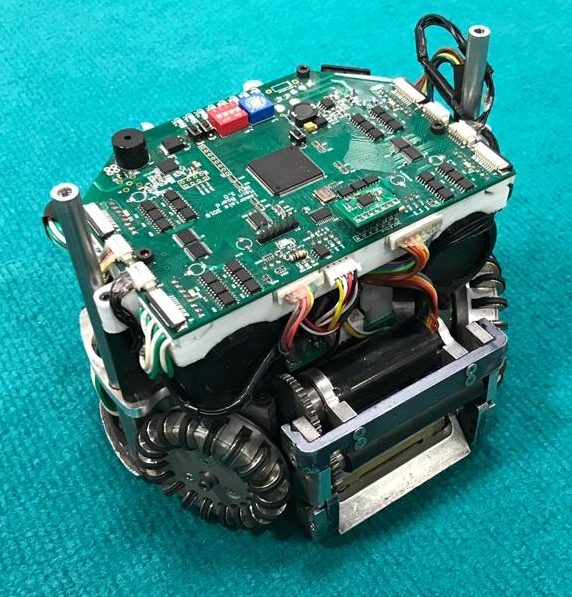
\includegraphics[width=10cm]{images/std_robot.jpeg}
\caption{Immortals current robot.} \label{fig_std_robot}
\end{figure}

This year the team had the chance to improve the AI software design which is the core program running on a desktop or laptop computer and is the means to navigate each robot. The robots move and take actions defined by this program. Other enhancements, however, have been continued to be made to the robots mechanics and electronics which will be explained further.

\section{Kicking System}
Before 2018 the limit for the ball velocity was 8m/s. In order for robots to kick a ball that much fast, a strong shooting system including capacitors and solenoids where required. Since RoboCup 2018, Montréal, Canada, the maximum speed limit has been decreased to 6.5m/s which makes teams to wonder if they want to redesign their robots kicking system and optimize the space consumption or battery power in their robot. This year the Immortals robots kicking system has been modified in order to optimize the energy consumption from the battery. This way robots have the chance to stay longer in a match without the need of their batteries to get changed.

\begin{figure}
\centering
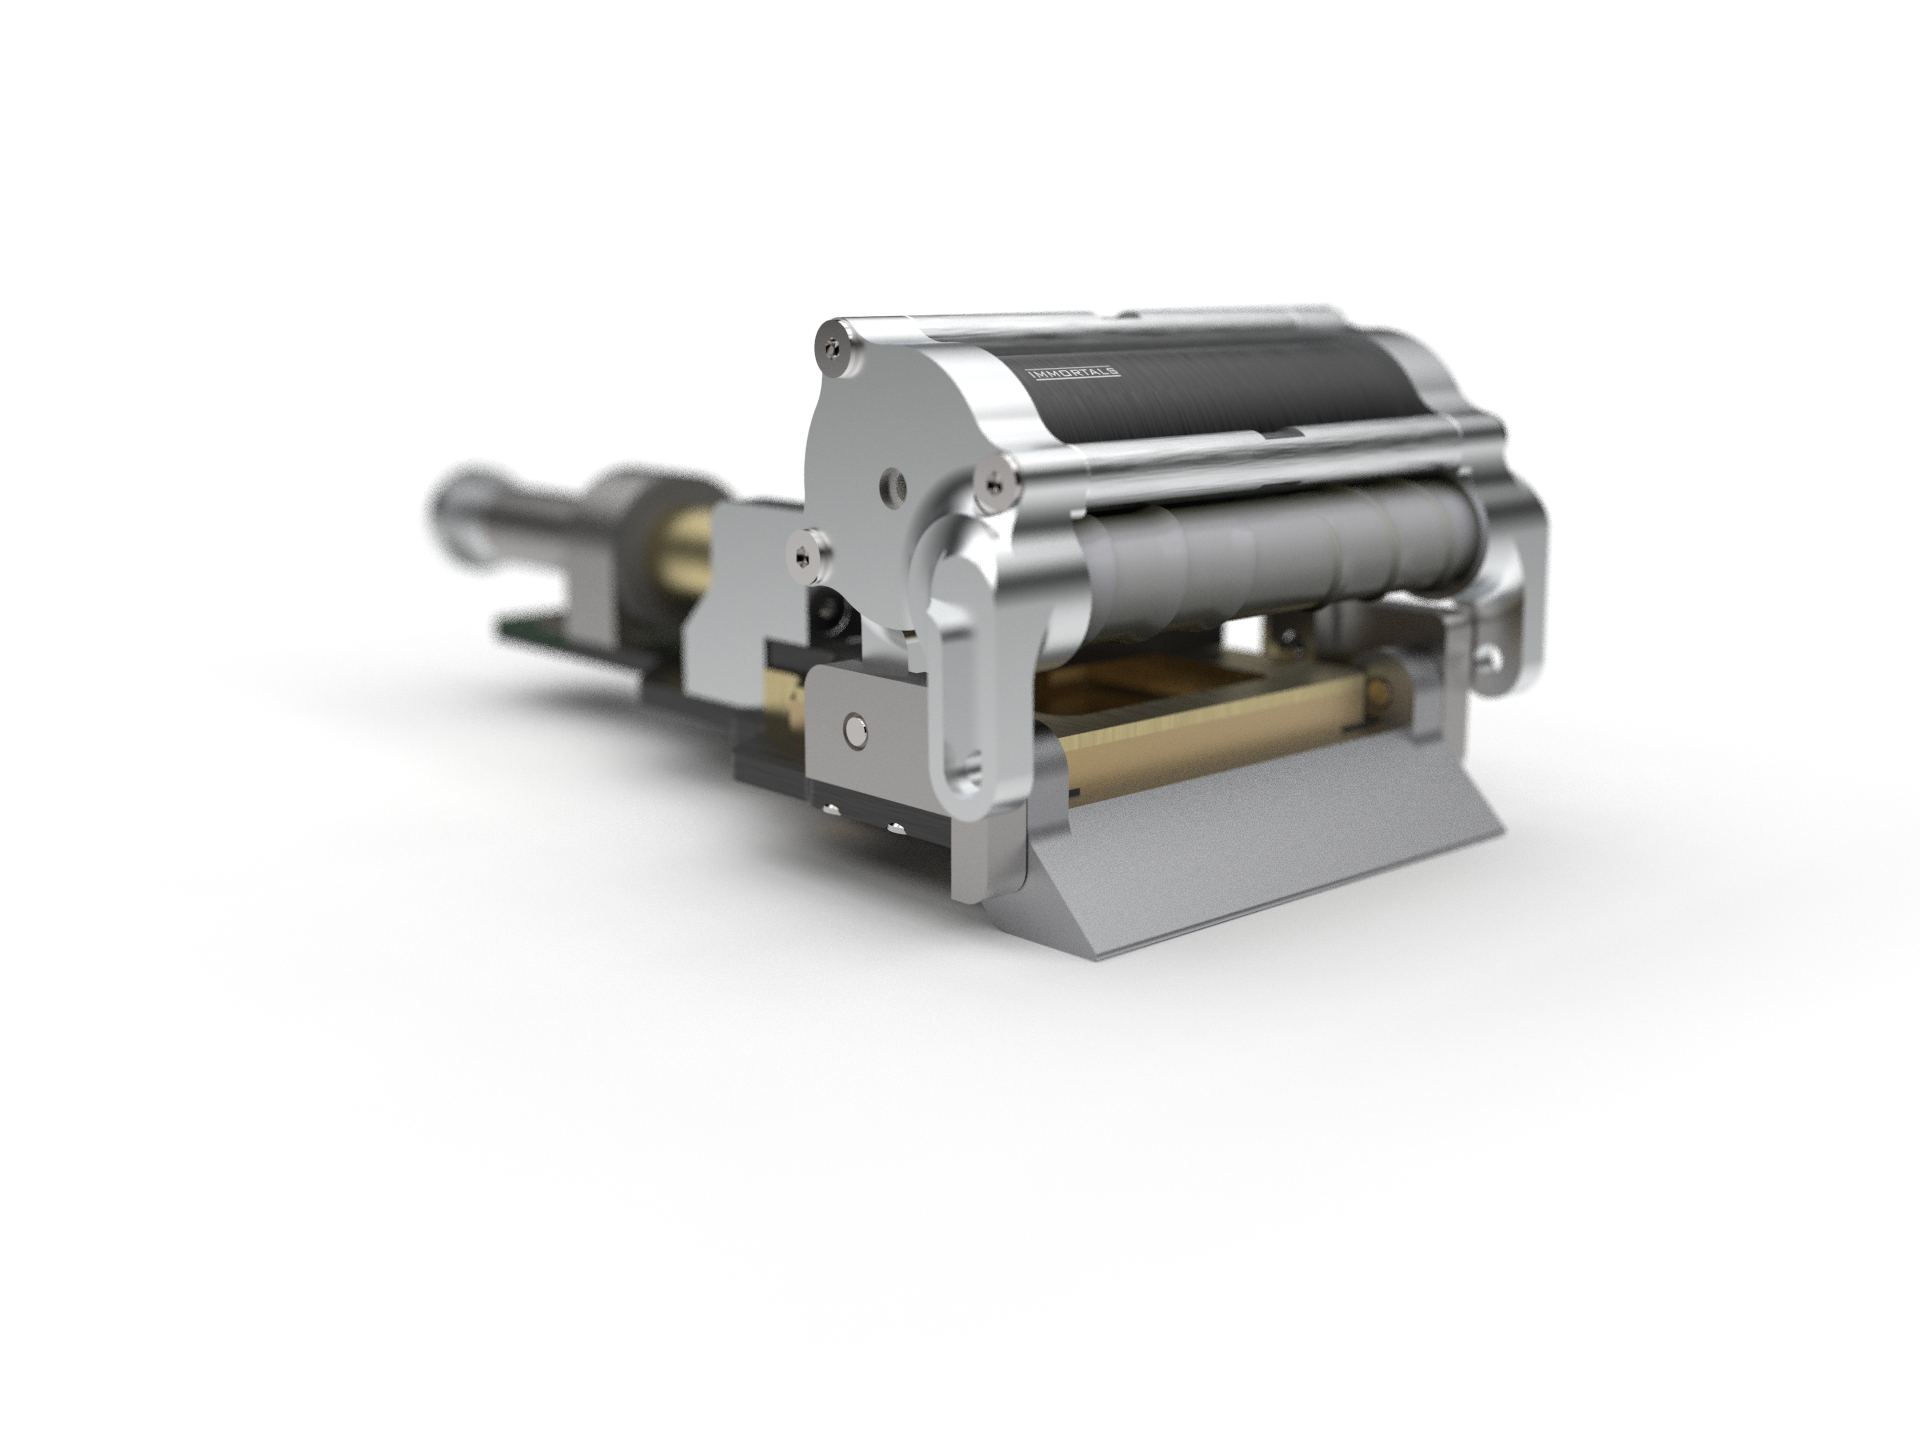
\includegraphics[width=10cm]{images/kicking_system.jpg}
\caption{The latest kicking system of the Immortals robots.} \label{fig_Kick_Sys}
\end{figure}

To understand the upgrade process of the shooting system, the reader is referred to the previous year (E)TDPs of this team~\cite{ref_ETDP2019,ref_ETDP2018}.

This year it has been decided to redesign the shooting solenoid which is the part that converts the electrical power to a magnetic field and thus it will move the metal plunger towards the ball to be kicked. The previous solenoid had a low resistance so a higher current will pass through it which will result in a higher speed. However, the kicking force will get a bit hard to control and it will generate a notable amount of heat. This part has been modified in a way that less current is flown in the solenoid to optimize energy consumption and generate less heat. Although the kicking power will decrease, it is still possible to kick the ball to more than 6.5m/s.

\section{Software}
This year the main software also known as the AI software is redesigned in order to be more understandable and extendable. In previous years the software core was the same for each year but with slight changes according to rules and new referee commands. The new members who wanted to implement a new idea in the software needed to spend a great amount of time to understand the methods to use for the robot navigation and data input.

The inputs for the software are vision data, referee commands and a configuration file which tells the initial parameter values for the network and match conditions. The outputs are simple navigation commands to the robots (e.g. moving with a given speed vector or kicking a ball with a specified amount of force).

The new software is written in C++ same as the previous one. The only reason to use this language is the performance and easy to extend capabilities of it. For example the ability to optimize the code by using GPUs are well known in this language.

\subsection{Finite-State Machine} 
After a few years of experience in the Small Size League as a software designer the key idea that every team is looking to implement is to make the robots to take the correct action at the exact time and condition. If the actions are performed correctly, the robots will accomplish their task which is scoring a goal or preventing the opponent from scoring. Unfortunately, there are many conditions that can happen in a match and each one has its own set of solutions these solutions are the sequence of commands which are given to a set of robots. For the software designer it may be hard to implement the solutions with a group of \textit{IF} conditions and no special structures.

In order to simplify the implementation for multiple software designers in the team, a Finite-State Machine implementation structure has been introduced. This gives a great flexibility and readability of implementation in the code. Each state is connected to other states by a condition or a set of conditions. This makes the implementation easier to probe. By tracking each state transition the faulty part of the code will be simply found.

Each state is basically a function which will be called whenever a complete picture of a field is received from the vision. The input of the function, or state, are the vision data.  
In each state, the set of commands which have to be given to the robots in the field are defined and if there is a condition which a state transition is required the next state will be defined to be called next time.
Table~\ref{tab1} shows a sample group of commands which can be used in every state:

\begin{table}[H]
\caption{Example commands which can be used in every state.}\label{tab1}
\begin{tabular}{|p{7.5cm}|p{6cm}|}
\hline
Function &  Explanation \\
\hline
{\itshape Navigate2Point(robot, destination, maxSpeed)} & Navigate the robot to a destination.\\
{\itshape ERRTNavigate2Point(robot, destination, maxSpeed)} & Navigate the robot while avoiding obstacles.\\
{\itshape Mark(robot, oppRobot)} & Position between the goal and an opponent robot.\\
{\itshape FetchBall(robot, point)} & Navigate the robot to a position on line which the ball is moving on and most close to the \textit{point}.\\
{\itshape OneTouchDirect(robot, point, target)} & Navigate the robot to a position on line which the ball is moving on and most close to the \textit{point}. Kick the ball towards the \textit{target}.\\
{\itshape CircleBall(robot, radius, angle)} & Position robot on a circle around the ball in a specific angle.\\
{\itshape Face(robot, point)} & Face the robot towards a point.\\
{\itshape Chip(robot, power)} & Robot should perform a chip kick whenever the ball was intercepted.\\
{\itshape Direct(robot, power)} & Robot should perform a direct kick whenever the ball was intercepted.\\
{\itshape CircleKickBall(robot, target, power)} & Position robot on a circle around the ball and towards the \textit{target}, then kick the ball.\\
%Title (centered) &  {\Large\bfseries Lecture Notes}\\
%1st-level heading &  {\large\bfseries 1 Introduction}\\
%2nd-level heading & {\bfseries 2.1 Printing Area}\\
%3rd-level heading & {\bfseries Run-in Heading in Bold.} Text follows\\
%4th-level heading & {\itshape Lowest Level Heading.} Text follows\\
\hline
\end{tabular}
\end{table}

As shown in Table~\ref{tab1} the commands are fairly simple to be understood. This simple implementation saves a great amount of time for the programmers to extend or debug the code.

\subsection{Debugging}
Another experience with the previous AI software was the process of debugging the algorithms and, in general, the code itself. To overcome this problem, a logging protocol has been implemented which defines the messages that are sent from the AI software while operating. Using that protocol, whenever a computer is running the AI software while connected to the network, any other computer in the same network can run a logging software and monitor the AI software's parameters including not just the simple inputs from the vision, but also the state, predictions of the algorithms and et al. Fig~\ref{fig_visualizer} shows the graphical visualizer which monitors and records the parameters in the AI software. The visualizer is implement in python while the AI is written in C++ as mentioned before.

\begin{figure}
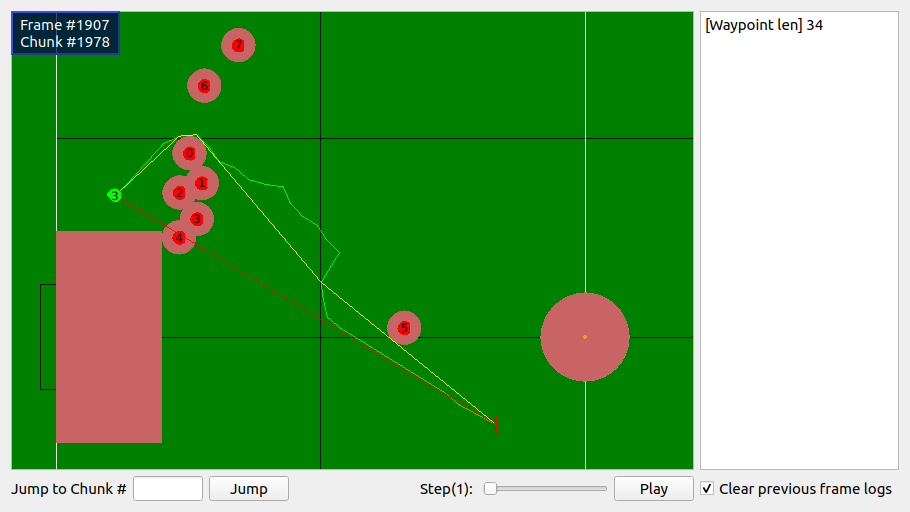
\includegraphics[width=\textwidth]{images/visual1.png}
\caption{A demonstration of the ERRT path plan in the graphical visualizer.} \label{fig_visualizer}
\end{figure}

Fig~\ref{fig1_plotter} shows a simple plotter which  visualizes the changes in the speed and commanded velocity of a single robot. This logging tool is also written in python.

\begin{figure}
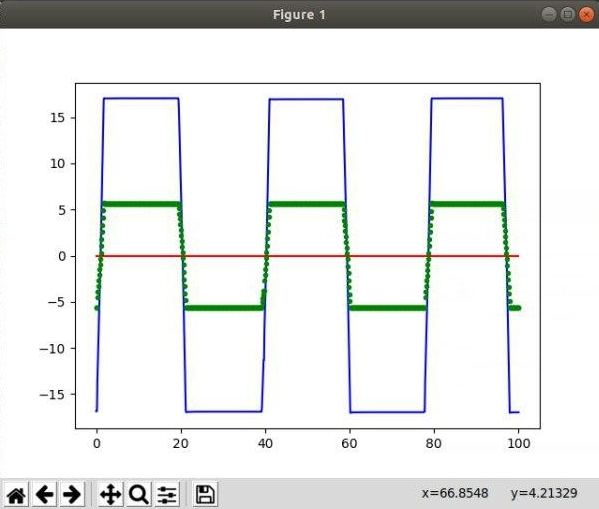
\includegraphics[width=\textwidth]{images/plotter.jpg}
\caption{An example logging program compatible with the new AI software.} \label{fig1_plotter}
\end{figure}

\subsection{Analyzing}
With the tools and designs which were introduced above, it is now possible to demonstrate different features of this project. Below, we will describe the analyzing process in the AI with an example. In the example the goal is to find the best spot in order for a robot to perform a one-touch kick\footnote{A one-touch kick is a robots action where a ball is kicked immediately it touches the front of the robot.}.

There are many parameters to notice while performing a successful one-touch kick (e.g. Initial Ball Velocity, Robots Angle, Velocity of the robot, Target position of the kick). A simple solution to find the optimum values for the parameters is to run tests with different initializations of the parameters. Here, the tests are performed in grSim~\cite{ref_grsim}.

For this example at first, a ball and two robots are stationed at defined locations and a target position is randomly picked in a defined window.

Second, after waiting for a while, one of the robots moves toward the ball and kicks it towards the target position. Meanwhile, the other robot tries to reach to the target position.

Third, After the ball has been moved the second robot is commanded to perform a one touch kick and direct the ball to the center of the goal. This process continues until the ball passes the fields side line or the ball stops moving. If the ball enters the goal, the target position is tagged as a success, in other cases it is tagged as a fail. After this the \textit{round} counter increases by one and the process is repeated from the first state.

At last, After 500 rounds the process is finished and the results are shown in the debugging tools (i.e. the graphical visualizer).

Fig~\ref{fig_ANALYZE_SING_ITR} shows how a single round is performed.

\begin{figure}
\centering
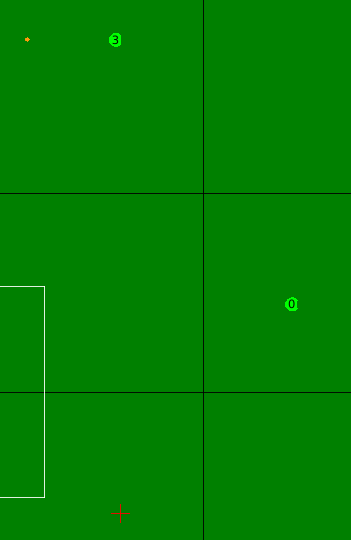
\includegraphics[height=5cm]{images/Analyze_State1.png}
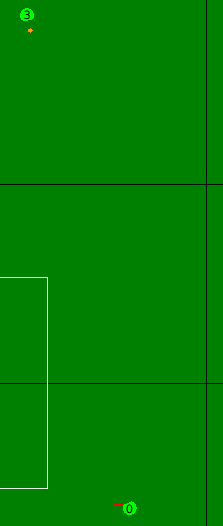
\includegraphics[height=5cm]{images/Analyze_State2.png}
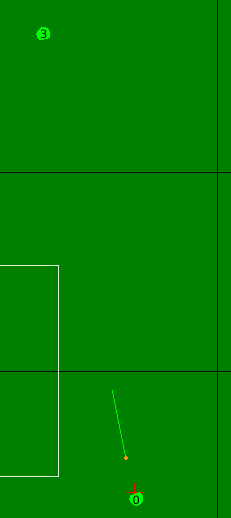
\includegraphics[height=5cm]{images/Analyze_State3.png}
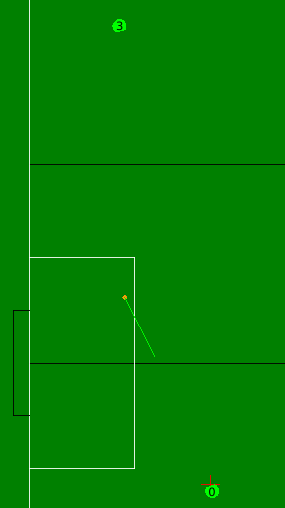
\includegraphics[height=5cm]{images/Analyze_State4.png}\caption{The analysis process shown in the graphical visualizer. Starting from left.} \label{fig_ANALYZE_SING_ITR}
\end{figure}

To define this process the FSM chart shown in Fig~\ref{fig_ANALYZE_FSM} can be implemented in the project\footnote{The chart was drawn in \url{creately.com}}.

\begin{figure}
\centering
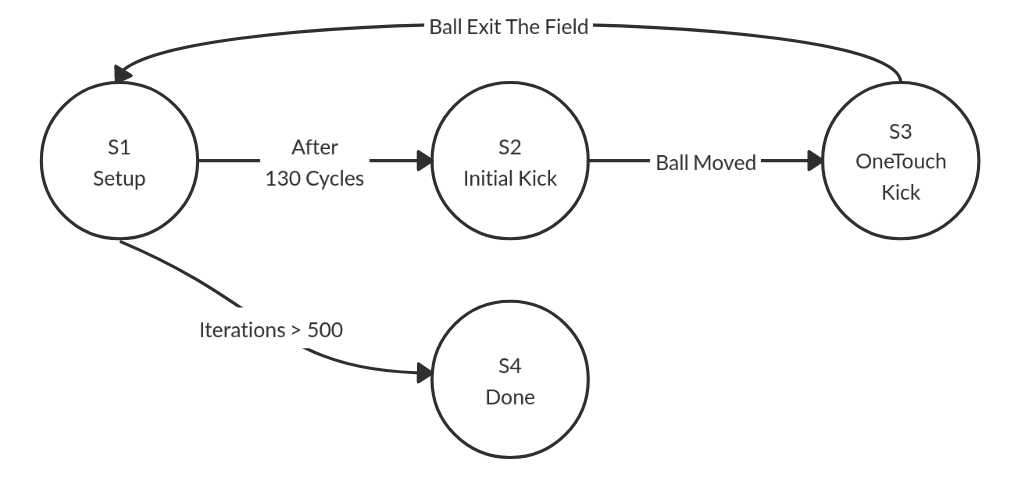
\includegraphics[width=10cm]{images/Analyze_FSM.png}\caption{The FSM chart for the analysis process.} \label{fig_ANALYZE_FSM}
\end{figure}

Now that the FSM is known, each state can be implemented. The pseudocodes of the states are defined in Tables~\ref{table_STATE1_IMP},~\ref{table_STATE2_IMP},~\ref{table_STATE3_IMP} and~\ref{table_STATE4_IMP}. These state functions have access to global variables which are defined in Table~\ref{table_GLOBAL_VARS}.

\begin{table}
\caption{Global variables of the FSM.}
\center
\label{table_GLOBAL_VARS}
\begin{tabular}{|p{10cm}|}
\hline
\textbf{var} 
targetPosition,
initRobotPositions,
initBallPosition,\\
\quad oppGoalPosition:Position;

\textbf{var}
round, cnt:int;

\textbf{var}
successPositions,failPositions:Position[];

\textbf{var}
nextFunc2Run:function;\\

\hline
\end{tabular}
\end{table}

In Table~\ref{table_GLOBAL_VARS}, the \textit{targetPosition} is the location where the robot will perform its one-touch kick. This variable is initialized in every round. 

The \textit{initRobotPositions} and \textit{initBallPosition} are the initial locations of the robots and the ball in every round. These variables are defined before the start of the test. \textit{oppGoalPosition} is the position of the center of the opponents goal line. This variable is defined before the start of the test.

\textit{successPositions} and \textit{failPositions} are two vectors which store the positions according to their tags, \textbf{fail} or \textbf{success}.

\textit{nextFunc2Run} is the function which will run in the next cycle (i.e. The next time a new vision dataset is received). This variable is defined as a C++ pointer to function in our executable code.


\begin{table}[H]
\caption{Implementation of the \textit{Setup} state.}
\center
\label{table_STATE1_IMP}
\begin{tabular}{|p{10cm}|}
\hline

\textbf{function}
$ S1\_setup$()\\
\quad placeRobots(initRobotPositions);\\
\quad placeBall(initBallPosition);\\
\quad targetPosition = pickRandomPosition();\\
\quad logData();\\
\quad \textbf{if} round >= 500 \textbf{then}\\
\quad\quad nextFunc2Run := S4\_done;\\
\quad\quad cnt := 0;\\
\quad \textbf{else if} cnt >= 130 \textbf{then}\\
\quad\quad nextFunc2Run := S2\_initKick;\\
\quad\quad cnt := 0;\\
\quad \textbf{else}\\
\quad\quad cnt := cnt + 1;\\

\hline
\end{tabular}
\end{table}

In \textit{S1\_setup}(), the robots and the ball have to get placed in the specified positions. This can be done by replacing the balls by hand or by robots and at last navigating the robots towards the specified positions.
If the test is being performed in a simulator (e.g. grSim) it is possible to immediately place the robot by a command. Since the current test is performed in grSim, the robots will be placed using the placement commands implemented in grSim. These commands are shown as \textit{initRobotPositions}() and \textit{initBallPosition}() in the pseudocode. In every cycle (i.e. every time the function is called) A variable called \textit{cnt} is incremented by one. It is checked in an if statement to check whether it is time to transit to the next state or to stay in the current state. Another if statement checks if the round number has reached to 500, if so, the FSM will transit to the \textit{done} state which brings the process to an end.

\begin{table}[H]
\caption{Implementation of the \textit{Initial Kick} state.}
\center
\label{table_STATE2_IMP}
\begin{tabular}{|p{10cm}|}
\hline

\textbf{function}
$ S2\_initKick$()\\
\quad circleKickBall(Robot3, targetPosition, 100);\\
\quad ERRTNavigate2Point(Robot0, targetPosition);\\
\quad logData();\\
\quad \textbf{if} cnt >= 5 \textbf{then}\\
\quad\quad nextFunc2Run := S3\_oneTouchKick;\\
\quad\quad cnt := 0;\\
\quad \textbf{else if} ballIsMoving() \textbf{then}\\
\quad\quad cnt := cnt + 1;\\

\hline
\end{tabular}
\end{table}

In \textit{S2\_initKick}(), Robot \#3 tries to aim the \textit{targetPosition} and kick the ball towards it. Meanwhile, Robot \#0 will try to reach the \textit{targetPosition}. After a few moments when the ball is moving, the FSM will transit to the next state.


\begin{table}[H]
\caption{Implementation of the \textit{OneTouchKick} state.}
\center
\label{table_STATE3_IMP}
\begin{tabular}{|p{10cm}|}
\hline

\textbf{function}
$ S3\_oneTouchKick$()\\
\quad halt(Robot3);\\
\quad oneTouchDirect(Robot0, targetPosition, oppGoalPosition);\\
\quad logData();\\
\quad \textbf{if} ballIsOut() \textbf{then}\\
\quad\quad \textbf{if} ballInGoal() \textbf{then}\\
\quad\quad\quad successPositions.add(targetPosition);\\
\quad\quad \textbf{else} \\ 
\quad\quad\quad failPositions.add(targetPosition);\\
\quad\quad nextFunc2Run := S1\_setup;\\
\quad\quad round := round + 1;\\
\quad \textbf{else if} ballIsNotMoving() \textbf{then}\\
\quad\quad failPositions.add(targetPosition);\\
\quad\quad nextFunc2Run := S1\_setup;\\
\quad\quad round := round + 1;\\

\hline
\end{tabular}
\end{table}

In \textit{S3\_oneTouchKick}(), Robot \#3 gets into a halt mode and Robot \#0 will wait for the ball to reach it. Once the ball gets fetched by the robot. it will get kicked towards the \textit{oppGoalPosition}. The state transition will not happen until the ball exits the field or stops moving. When one of the transition conditions happen it will be judged whether the test was a success or a fail according to the position of the ball in relation with the goal.

\begin{table}[H]
\caption{Implementation of the \textit{Done} state.}
\center
\label{table_STATE4_IMP}
\begin{tabular}{|p{10cm}|}
\hline

\textbf{function}
$ S4\_done$()\\
\quad halt(Robot3);\\
\quad halt(Robot0);\\
\quad logData();\\
\quad logData(successPositions, GREEN);\\
\quad logData(failPositions, RED);\\

\hline
\end{tabular}
\end{table}

In \textit{S4\_done}(), the robots are halted and the results are sent to the visualizer as red and green points.

After running the code with 500 rounds in 1 hour and 20 minutes, the results were shown on the visualizer with 142 successful and 358 failed attempts. Fig~\ref{fig_ANALYZE_OUTPUT} shows the visualizer at the end of the test. It is now clearly seen which areas have a high possibility in scoring a goal by a one-touch kick under the tested conditions.

\begin{figure}[H]
\centering
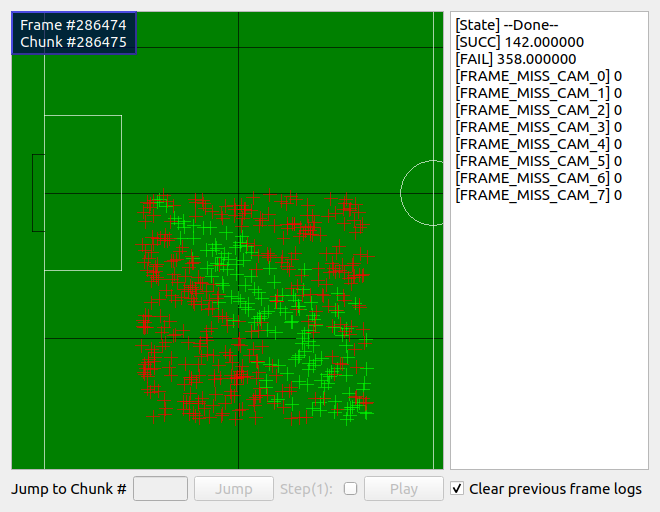
\includegraphics[width=10cm]{images/Analyze_output.png}\caption{The final results of the analysis.} \label{fig_ANALYZE_OUTPUT}
\end{figure}

Finally, it is worth to notice that the test has been performed in a simulation to give a better result in a short amount of time. It is clear that this test has to be made on robots in the real world. In that case, the number of rounds will obviously need to decrease to a few tens. The focus of this section was to show how an analysis procedure is taken in the Immortals AI project.

%\section{3D printed robot}
%As mentioned in the previous years team description papers~\cite{ref_ETDP2019,ref_ETDP2018}, A new type of robot was introduced to the league by this team in order to reduce the time and energy for manufacturing the robots.
%
%The design of the 3d printed robots where published and are available for teams and individuals to use~\cite{ref_opensource}. The designs are being updated to increase robustness. However, the robustness of a 3d printed robot is incomparable with a usual SSL robot which is assembled with metal parts. Teams may choose to build this type of robot in order to run tests which require a high number of robots.

%\begin{figure}
%\centering
%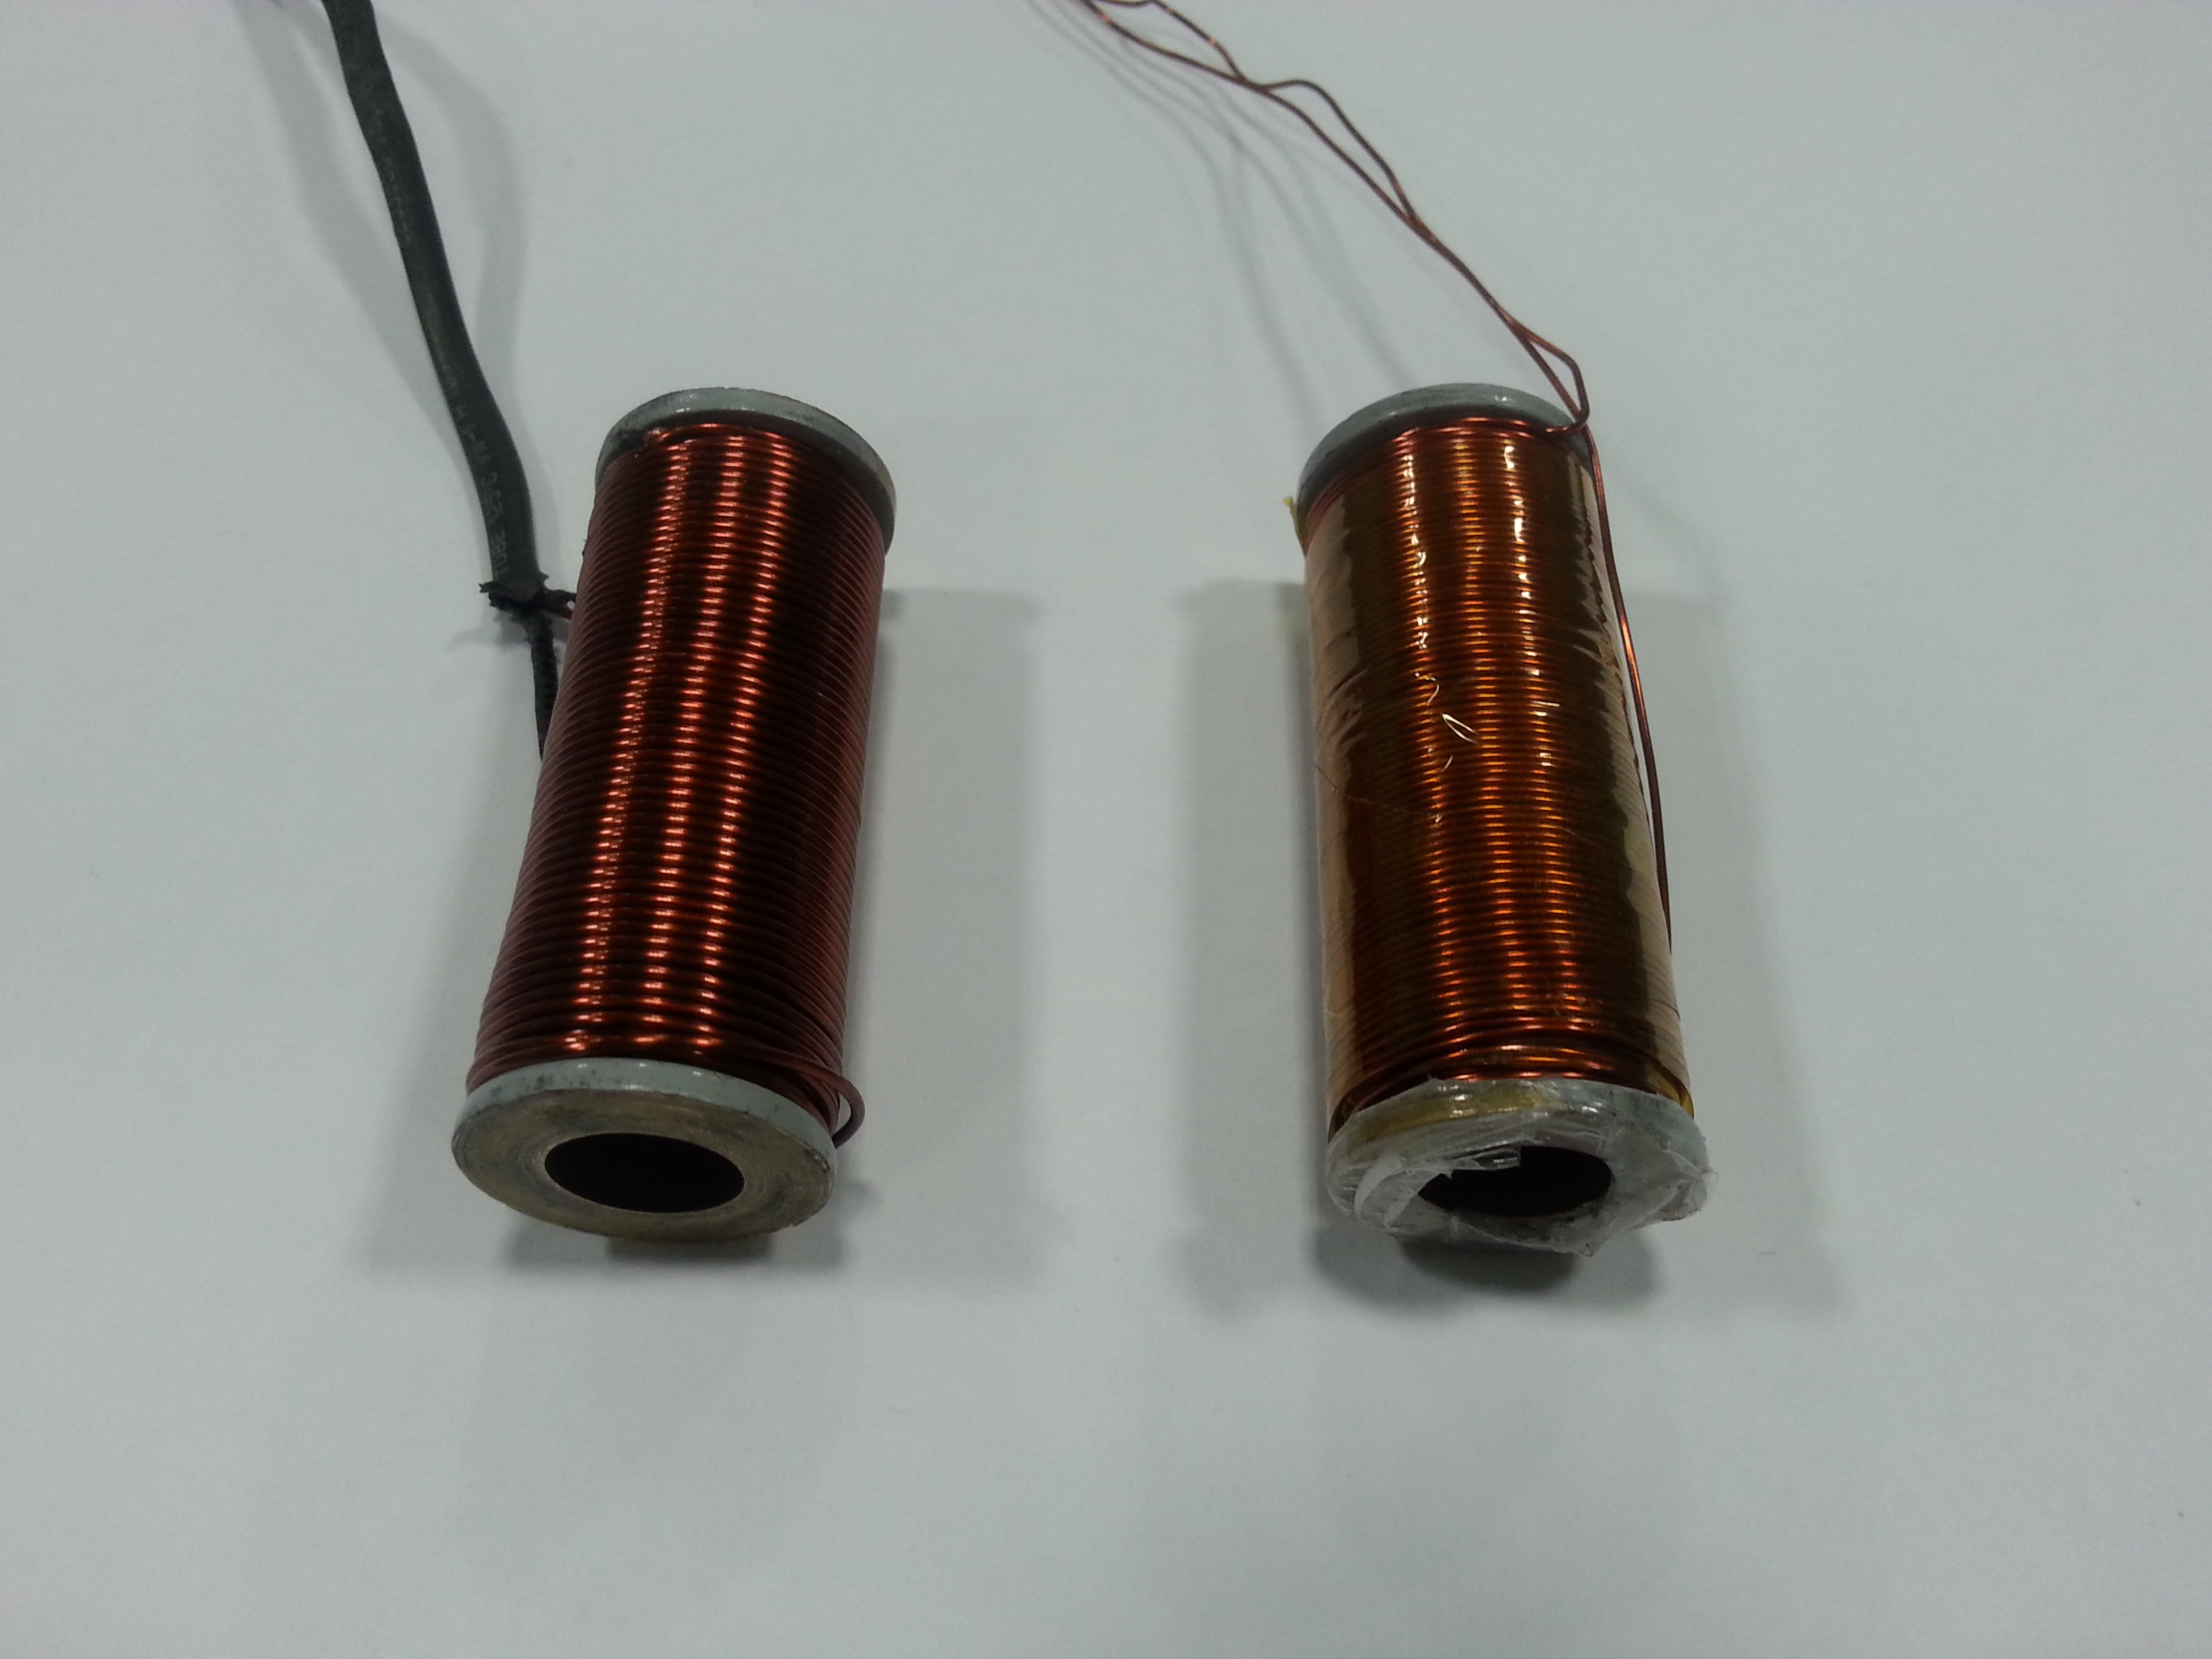
\includegraphics[width=10cm]{images/solenoid.jpg}
%\caption{The old solenoid(Left) and the new solenoid(Right).} \label{fig_solenoid}
%\end{figure}


%\begin{figure}
%\centering
%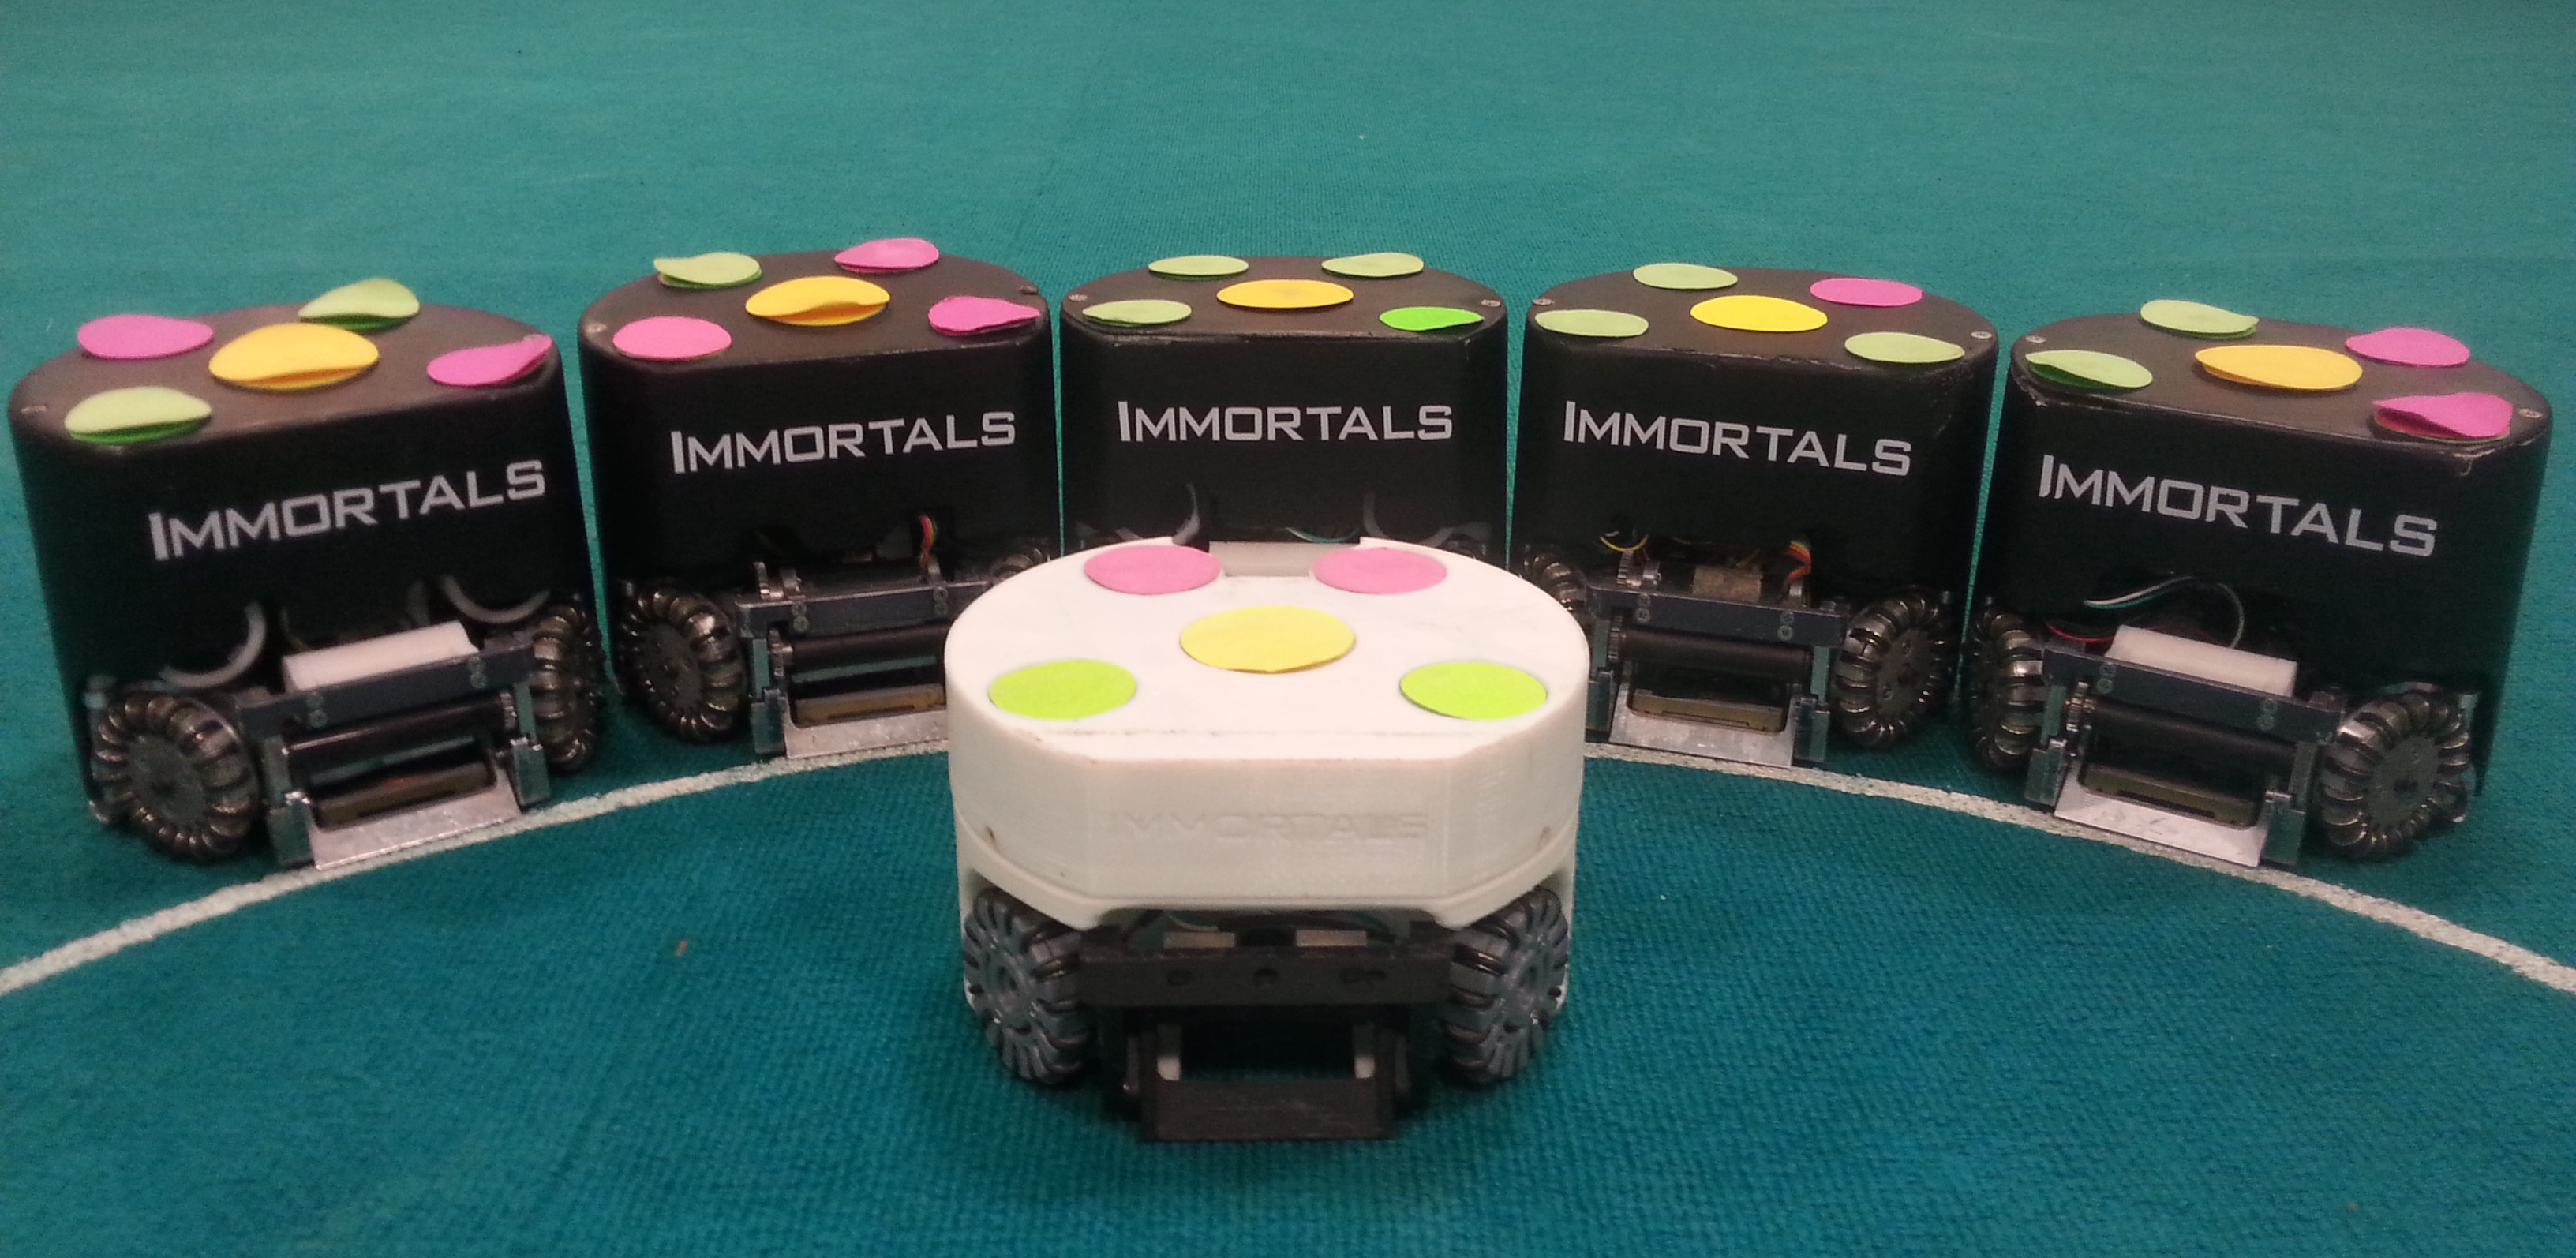
\includegraphics[width=10cm]{images/5plus1.jpg}
%\caption{Five old robots and a single 3D printed robot at the front.} \label{fig_5plus1}
%\end{figure}



\newpage
\begin{thebibliography}{8}
\bibitem{ref_website}
Immortals Robotics Website, \url{http://www.immortals-robotics.com}.

\bibitem{ref_ETDP2019}
Immortals 2019 Team Description Paper, \url{https://ssl.robocup.org/wp-content/uploads/2019/03/2019\_ETDP\_Immortals.pdf}.

\bibitem{ref_ETDP2018}
Immortals 2018 Team Description Paper, \url{https://ssl.robocup.org/wp-content/uploads/2019/01/2018\_TDP\_Immortals.pdf}.

\bibitem{ref_opensource}
Immortals Open Source Project. \url{https://github.com/Ma-Ghasemieh/Immortals\_ssl\_opensource\_mech}.

\bibitem{ref_opensource}
Immortals Open Source Publish in RoboCup 2016. \url{https://github.com/lordhippo/immortalsSSL}.

\bibitem{ref_grsim}
Monajjemi, Valiallah (Mani), Ali Koochakzadeh, and Saeed Shiry Ghidary. "grSim – RoboCup Small Size Robot Soccer Simulator." In Robot Soccer World Cup, pp. 450-460. Springer Berlin Heidelberg, 2011.

\end{thebibliography}
\end{document}
